Power of laser light
\begin{align*}
P = 1 \text{mW}
\end{align*}

Output current of photodiode (consider the best case: no power loss during transmission)
\begin{align*}
I = 0.8 P
\end{align*}

Output power of photodiode
\begin{align*}
P_{out} &= I^2 R = 0.64 P^2 R
\end{align*}

Consider \textbf{conservation of energy} (the photodiode can only obtain energy from the laser light)
\begin{align*}
&P_{out} = 0.64 P^2 R \le P\\
&R \le \frac{1}{0.64P} = 1562.5 \Omega
\end{align*}

Apparently, the photodiode is a current source with \textbf{voltage} upper bound.

\begin{align*}
V_{\max} = 1562.5 \times 0.8 P = 1.25 \text{V } (= 0.8^{-1})
\end{align*}
Output voltage is not high enough to reach \texttt{digitalRead()} HIGH (3V) or to trigger an external interrupt. As a result, operational amplifiers need to be implemented.\\

The code written in last year\\
\url{https://github.com/leeang/Electronic-System-Implementation/blob/master/past%20paper/2014%20Q2.c}

Pretty similar to 2013 Q2.

\begin{figure}[H]
\centering
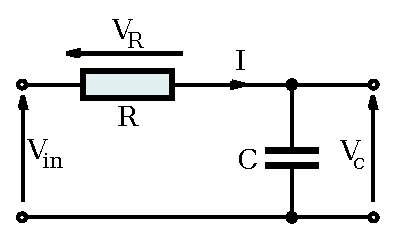
\includegraphics[width=0.3\linewidth]{RC}
\end{figure}

\textbf{Useful Equation}
\begin{align*}
V_C(t) = V_0 (1 - e^{-\frac{t}{RC}})
\end{align*}

When $t = RC$,
\begin{align*}
V_C(t)|_{t=RC} = V_0 (1 - e^{-1}) = 0.632 V_0
\end{align*}

Supply $V_0$ = 5V from $t=0$ and the capacitor starts charging.\\
Record 1st timestamp \texttt{t1 = micros();}\\

\texttt{analogRead()} the voltage across the capacitor $V_C$ until $V_C(t) = 0.632 V_0$\\
Record 2nd timestamp \texttt{t2 = micros();}.\\

Charing time $\tau$ = \texttt{(t2 - t1) / 1E6;} $\Longrightarrow$ $C = \frac{\tau}{R}$.\\

Thus the temperature can be calculated from $C$.\\

Be careful. The return value of \texttt{micros()} is enormous. (Unit: microsecond)\\
Please declare the variable as \texttt{unsinged long t = micros();}.
